% TODO fill in your paper title
\newcommand{\PaperTitle}{Simple Model Assemblages for Website Identification}
% TODO fill in your paper number when you get it
% \newcommand{\PaperNumber}{XXX}

\documentclass[10pt,sigconf,letterpaper,nonacm]{acmart}

%%%%%%%%%%%%%%%%%%%%%%%%%%%%%%%%%%%%%%%%%%%%%%%%%%%%%%%%%%%%%%%%%%%%%%%%%%%%
% This is the preamble; include packages as you see fit.
% Here are a few recommendations:
% \usepackage{color}
\usepackage{graphicx}
% \usepackage[labelformat=simple]{subcaption}
% \usepackage{xspace}
% \usepackage{multirow}
% \usepackage[ruled,vlined]{algorithm2e}
% \usepackage{ulem}
\usepackage{url}
% \normalem

%%%%%%%%%%%%%%%%%%%%%%%%%%%%%%%%%%%%%%%%%%%%%%%%%%%%%%%%%%%%%%%%%%%%%%%%%%%%

\begin{document}

\title{\PaperTitle}

\author{Charles Hu}
\email{czhu06@wm.edu}
\affiliation{
  \institution{William \& Mary}
  \city{Williamsburg}
  \state{Virginia}
  \country{USA}
}

\begin{abstract}
  A clear and well-documented \LaTeX\ document is presented as an
  article formatted for publication by ACM in a conference proceedings
  or journal publication. Based on the ``acmart'' document class, this
  article presents and explains many of the common variations, as well
  as many of the formatting elements an author may use in the
  preparation of the documentation of their work. A cite so this compiles.
\end{abstract}

\keywords{Network trafifc, Network traffic classification, Machine learning, Ensemble models}

\maketitle

\section{Introduction}


\section{Proposed Method}

The following section details the design and rationale behind the methodology used for evaluating and classifying the website of origin for given samples of web traffic using machine learning models.

\subsection{Data Preparation}

In order to ensure that our developed models are robust and effective at their classification task, we employ a measured and systemized approach towards data collection and preprocessing to ensure that possibility of gathering ideosyncratic or erroneous data is minimized as much as possible.

The primary objective during the design of the data preparation phase was to ensure that the generated data set allows us to construct models that are effectively generalizable and not too overfit.
A key principle that allows us to achieve this is confirming that the gathered sample is as representative as possible of the general population; however, this is difficult to verify empiricaly given the complex nature of the overall population.
As a result, a preemptive approach was taken which resulted in the design of a two-stage data preparation phase comprised of a precautious data collection stage and a mitigative data preprocessing stage.

\subsubsection{Data Collection}
Data collection is performed through the monitoring of artificial website activity aimed at emulating real user interactions common to the sampled websites.
Website traffic between the user and the server hosting the website is monitored and tracked using Wireshark, an open-source software used for network traffic capture and analysis \cite{wireshark}.
Wireshark will specifically target the transport layer of network communication and intercept ongoing TCP streams between the user and the site host.
Activity on a website will occur through the controlled usage of a website's typical functionalities.
For instance, on a streaming site, the data collector will utilize the site's recommendation algorithm to view a certain number of videos before halting activity.
The goal during the activity substage is to interact with the website in a naturalistic manner akin to any typical user but avoid operations which either go beyond the scope of the target website (e.g., entering another website through an embedded link) or are unexpected of a user (e.g., manually performing HTTP operations with the website or abruptly closing the site during an interaction).
These precautions should help minimize the amount of collected TCP streams that contain information that are erroneous or overly noisy.
Once activity on a website has been concluded, Wireshark will be used to display the TCP streams generated during activity with the website (as seen in Fig. ~\ref{fig:wireshark}) and will export the TCP streams to an external CSV file for each targeted website.

\begin{figure*}[h]
  \centering
  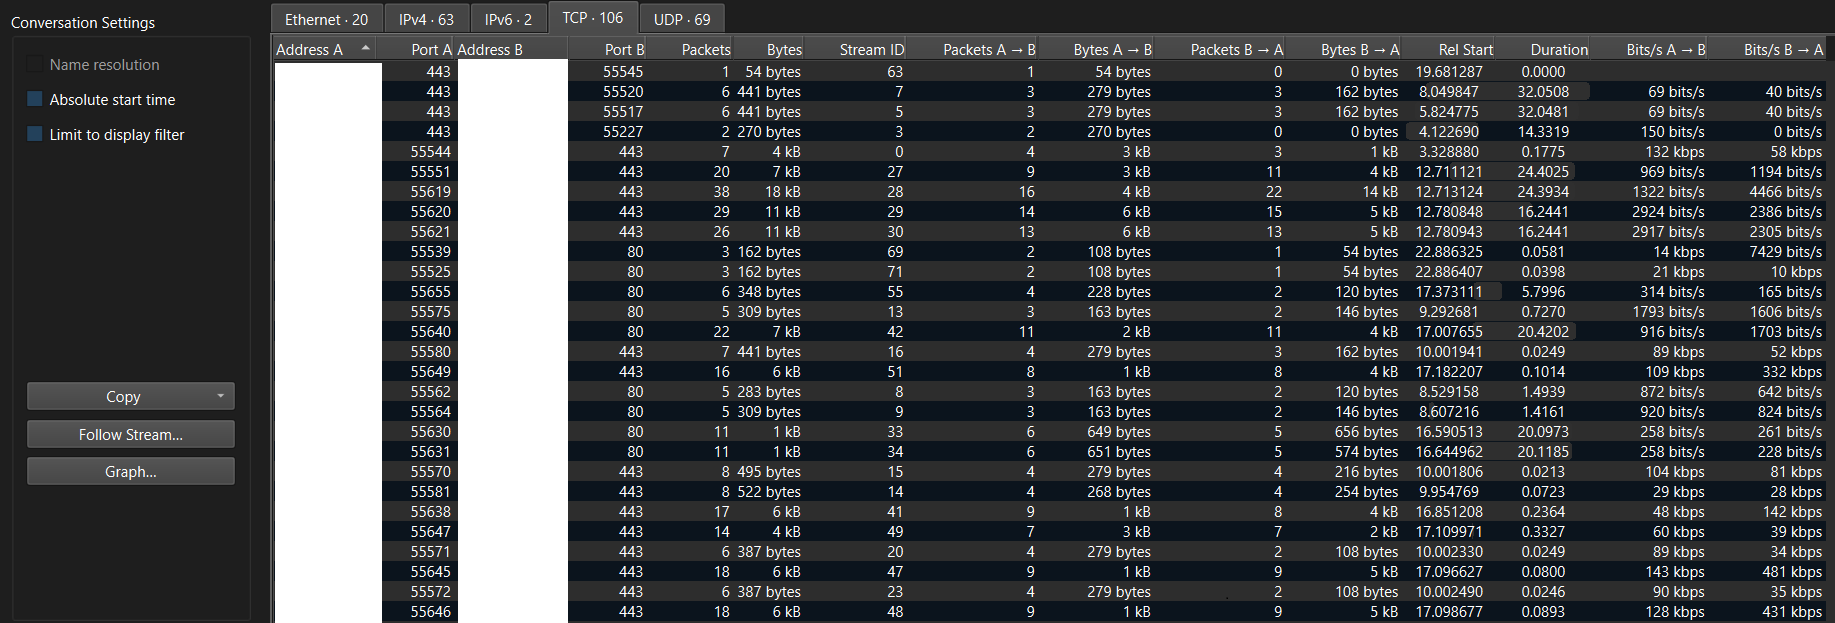
\includegraphics[width=.9\pdfpagewidth]{img/wireshark.png}
  \caption{A Wireshark window displaying tracked TCP streams and each stream's corresponding attributes. Note that IP addresses have been censored.}
  \label{fig:wireshark}
\end{figure*}

\subsubsection{Data Preprocessing}
Data preprocessing involves pruning the resulting data set from the data collection stage to remove features that are either explicitly detrimental or extraneous.
The removal of these features help improve the generalizability of our developed models by decreasing the overall model complexity and thus the variance inherent to it \cite{introInfo}; thus, if any idiosyncrasies or noise make it through our first stage of data collection, we can still reduce their influence on the overall model performance by lowering the capacity of the model to learn bad data.
To ensure that we do not develop models that have too low complexity due to a lack of learned features (and therefore trending towards too much bias in the bias-variance tradeoff), only features that are explicitly detrimental or extraneous will be removed.
Removed features are as follows:

\begin{itemize}
  \item \textbf{Address A, Port A, Address B, Port B}: These feature are explicit identifiers for the hosts in the TCP stream. Their inclusion would make the classification task redundant and would result in a model that places high importance on observing the IP and port values over other potentially useful features.
  
  \item \textbf{Stream ID}: This feature tracks the unique internal tracking ID given by Wireshark to any given TCP stream for later reference. This is Wireshark specific and not pertinent to the TCP stream itself.
  
  \item \textbf{Total Packets, Percent Filtered}: These features refer to the fitler display feature in Wireshark which filters every available packet to search for some filter specification (in this case, the target website). These are Wireshark specific and not pertinent to the TCP stream itself.
  
  \item \textbf{Rel Start}: This feature indicates when the TCP stream began relative to the start of the Wireshark network capture session. This is Wireshark specific and not pertinent to the TCP stream itself.
\end{itemize}

Retained features from the data set demonstrate either potential for aiding a model in identifying what a particular website is or are neutral in their benefit and do not actively harm or mislead the model in any way.
Retained features from the raw data set are as follows:

\begin{itemize}
  \item \textbf{Packets}: This feature tracks the total packets transferred. Note that since this is a TCP stream, this feature instead referes to a TCP segment. Different website functionalities may result in different tendencies in frequency and amount of segments transferred during a TCP stream.
  
  \item \textbf{Bytes}: This feature tracks the total amount of data in bytes that have been transferred during the entire TCP stream. Different website functionalities may result in smaller or larger sized data payloads being sent across the TCP stream.
  
  \item \textbf{Packets A $\rightarrow$ B, Bytes A $\rightarrow$ B}: These features track the packet count and total amount of data in bytes being sent from host A (the user) to host B (the site host). How intensive interactions between the user and the website are may influence these features.
  
  \item \textbf{Packets B $\rightarrow$ A, Bytes B $\rightarrow$ A}: These features track the packet count and total amount of data in bytes being sent from host B (the site host) to host A (the user). How intensive interactions between the website and the user are may influence these features.
  
  \item \textbf{Duration}: The entire time duration of the TCP stream recorded in seconds. Different durations may help indicate the purpose and level of engagement for a website.
  
  \item \textbf{Bits/s A $\rightarrow$ B, Bits/s B $\rightarrow$ A}: These features track the bitrate of the TCP stream. These features may not necessarily help the model as bitrate is subject to a number of factors that cannot be consistently attributed to a website alone, but the feature itself is not inherently detrimental so it has been left in the data set.
\end{itemize}

\subsection{Data Specifications}

\subsubsection{Data Analysis}

\subsection{Model Development}

\subsection{Model Specifications}

\subsubsection{Simple Models}

\subsubsection{Ensemble Models}


\section{Evaluation}

\subsection{Evaluation Metric}

\subsection{Results}

\subsubsection{Baseline}

\subsubsection{Simple Model Results}

\subsubsection{Ensemble Model Results}

\subsubsection{Model Results Overall}


\section{Discussion \& Future Work}

\subsection{Result Interpretations}

\subsection{Future Work}


\section{Conclusion}


% Note from the CFP that this section must include a statement about
% ethical issues; papers that do not include such a statement may be
% rejected.

%%%%%%%%%%%%%%%%%%%%%%%%%%%%%%%%%%%%%%%%%%%%%%%%%%%%%%%%%%%%%%%%%%%%%%%%%%%%
% We're in the endgame now

\bibliographystyle{ACM-Reference-Format}
\nocite{*}
\bibliography{refs}

\end{document}
